\documentclass[UTF8, heading=true]{ctexart}
\usepackage{karnaugh-map}
%-----中文宏包-----
\usepackage[UTF8]{ctex}
\usepackage[utf8]{inputenc}
\usepackage{titling}
%-----数学宏包-----
\usepackage{amsmath,amsthm,amssymb,amsfonts}
\usepackage{mathrsfs,bm}
\usepackage{dirtree}
%-----draft下 label提示-----
%\usepackage[notcite,notref]{showkeys}
%-----页面布局-----
\usepackage{geometry}
\geometry{left=1.25in,right=1.25in,top=1in,bottom=1in}
%\geometry{left=1in,right=1in,top=1in,bottom=1in}
%\geometry{left=2.5cm,right=2.1cm,top=1.7cm,bottom=2cm,includehead,includefoot}

%-----设置超链接-----
\usepackage{url,hyperref}
\hypersetup{colorlinks=true,linkcolor=black,citecolor=black} % 去掉目录红框
%-----制作目录-----
\usepackage{imakeidx}
% 设置颜色
% \usepackage{color,xcolor}
% 插入图片
\usepackage{graphicx}
\usepackage{epsfig}
%-----设置表格-----
\usepackage{tabularx,array}
\usepackage{longtable}
\usepackage{booktabs}
\usepackage{multirow}
\usepackage{multicol}
\usepackage{fancybox}
%-----调整单元格格式-----
\usepackage{makecell}
%-----操作字符串-----
\usepackage{xstring}
%-----设置章节标题和目录-----
\usepackage{titletoc}
\usepackage{titlesec}
%-----数学公式扩展-----
\usepackage{mathtools}
%-----浮动体设置-----
\usepackage{float}
%-----书签设置-----
\usepackage{bookmark}
%-----参考文献格式-----
\usepackage[numbers]{natbib}
%-----设置页眉页脚格式-----
\usepackage{fancyhdr}
% --- 设置代码环境 -----
\usepackage{color,xcolor}
\usepackage{listings}
\definecolor{bg}{rgb}{0.95, 0.95, 0.95}
\definecolor{keywordcolor}{rgb}{0.0, 0.0, 0.5}
\definecolor{commentcolor}{rgb}{0.0, 0.5, 0.0}
\definecolor{stringcolor}{rgb}{0.6, 0.1, 0.0}

% 设置 listings 样式
\lstdefinestyle{cppstyle}{
    language=C++,
    backgroundcolor=\color{bg},
    basicstyle=\small\ttfamily,
    keywordstyle=\color{keywordcolor}\bfseries,
    commentstyle=\color{commentcolor}\itshape,
    stringstyle=\color{stringcolor},
    numbers=left,
    numberstyle=\tiny\color{gray},
    numbersep=5pt,
    frame=lines,
    breaklines=true,
    breakatwhitespace=false,
    tabsize=4,
    showtabs=false,
    showspaces=false,
    showstringspaces=false,
    captionpos=b,
    keepspaces=true,
    columns=flexible,
    xleftmargin=2em,
    framexleftmargin=1.5em,
    framexrightmargin=0.5em,
    framesep=2mm,
    escapeinside={(*@}{@*)},
    morekeywords={glm, VertexData, Vector3f, Vector4f, Eigen, auto}
}

\lstdefinestyle{pythonstyle}{
    language=Python,
    backgroundcolor=\color{bg},
    basicstyle=\small\ttfamily,
    keywordstyle=\color{keywordcolor}\bfseries,
    commentstyle=\color{commentcolor}\itshape,
    stringstyle=\color{stringcolor},
    numbers=left,
    numberstyle=\tiny\color{gray},
    numbersep=5pt,
    frame=lines,
    breaklines=true,
    breakatwhitespace=false,
    tabsize=4,
    showtabs=false,
    showspaces=false,
    showstringspaces=false,
    captionpos=b,
    keepspaces=true,
    columns=flexible,
    xleftmargin=2em,
    framexleftmargin=1.5em,
    framexrightmargin=0.5em,
    framesep=2mm,
    escapeinside={(*@}{@*)},
    morekeywords={import, from, def, class, if, else, for, while, return}
}

\lstset{style=cppstyle}

% ---- 定义列表项的样式 -----
\usepackage{enumitem}
\setlist{nolistsep}
% --- 设置英文字体 -----
\usepackage{fontspec}
\setmainfont{Times New Roman}
\usepackage{setspace}

\geometry{
  left=3.0cm,        % 左边距
  right=3.0cm,       % 右边距
  top=2.5cm,         % 上边距
  bottom=2.0cm       % 下边距
}
\renewcommand*{\baselinestretch}{1.5}
\newcommand{\upcite}[1]{\textsuperscript{\textsuperscript{\cite{#1}}}}

\renewcommand{\thesection}{\chinese{section}、}
\renewcommand{\thesubsection}{（\chinese{subsection}）}
\renewcommand{\thesubsubsection}{\arabic{subsubsection}.}
\titleformat{\section}{\bfseries \zihao{-3}}{\chinese{section}、}{0em}{}
\titleformat{\subsection}{\bfseries \zihao{4}}{（\chinese{subsection}）}{0.2em}{}
\titleformat{\subsubsection}{\bfseries \zihao{-4}}{\arabic{subsubsection}、}{0.2em}{}
\newcommand{\stunum}[1]{\def\defstunum{#1}}
\newcommand{\class}[1]{\def\defclass{#1}}

% ----- 设置浮动体间距 ------
\setlength{\textfloatsep}{0pt}
\setlength{\floatsep}{10pt plus 3pt minus 2pt}
\setlength{\intextsep}{10pt}
\setlength{\abovecaptionskip}{2pt plus1pt minus1pt}
\setlength{\belowcaptionskip}{3pt plus1pt minus2pt}

% ----- 设置公式间距为零 ------
\AtBeginDocument{
	\setlength{\abovedisplayskip}{4pt plus1pt minus1pt}
	\setlength{\belowdisplayskip}{4pt plus1pt minus1pt}
	\setlength{\abovedisplayshortskip}{2pt}
	\setlength{\belowdisplayshortskip}{2pt}
	\setlength{\arraycolsep}{2pt}   % array中列之间空白长度
}



% --- 自定义命令 -----
\newcommand{\CC}{\ensuremath{\mathbb{C}}}
\newcommand{\RR}{\ensuremath{\mathbb{R}}}
\newcommand{\A}{\mathcal{A}}
\newcommand{\ii}{\bm{\mathrm{i}}\,}  % 虚部
\newcommand{\md}{\mathrm{d}\,}
\newcommand{\bA}{\boldsymbol{A}}
\newcommand{\red}[1]{\textcolor{red}{#1}}
\graphicspath{{./img/}}

\pagestyle{fancy}
\fancyhf{}
\fancyfoot[C]{\thepage}
\fancyhead[L]{多模态最终报告}
\fancyhead[R]{文档理解+多模态检索问答系统}
\title{\LARGE \textbf{多模态最终报告 \hspace{0.2cm} 文档理解+多模态检索问答系统}}
\date{}
\author{小组成员1：庄仕豪 \qquad 学号：23336355 \\ 小组成员2: 钟晨晖 \qquad 学号：23336336}

\begin{document}
\maketitle
\vspace{-1.5cm}

% ================================================================
%  摘要
% ================================================================
\begin{abstract}
本文提出并实现了一套面向复杂版面 PDF 文档的多模态检索增强生成（Multimodal RAG）系统 MultimodalQA。
系统以 IBM Docling 完成 PDF 版面分析与结构化抽取（文本块 / 表格 Markdown / 图像裁剪），
以智谱 GLM-4.6V 生成图表语义摘要，以 BAAI/BGE-M3 构建 1024 维稠密向量索引（ChromaDB 持久化），
并通过 Multi-Vector Retriever 实现"摘要召回、原图回传"的代理检索策略，
最终由 GLM-4.6V 生成带页码与图号引用的多模态答案。

为定量评估系统优势，本文构建了一个包含 \textbf{200 道题目、5 篇文档、4 类领域、3 档难度}的自建 QA 数据集，
设计三路基线对比：多模态 RAG（完整系统）、纯文本保守基线（无图、无证据则拒答）、纯文本开放基线（无图、允许基于上下文推断），
以 ANLS 与准确率为指标进行评测。
实验结果表明，在必须依赖图表视觉信息的题目上（100 道），
多模态 RAG 的准确率（65\%）显著高于纯文本保守基线（18\%）和纯文本开放基线（42\%），
提升分别为 +47 个百分点（pp）和 +23 pp（McNemar 检验 $p<0.0001$），
而在纯文本题目上三路无显著差异，验证了多模态架构的必要性与针对性。

系统已实现完整的 Web 前后端（Vue 3 + FastAPI），
支持 PDF 拖拽上传、实时进度推送（SSE）、LaTeX 公式渲染与引用溯源。
\end{abstract}

\tableofcontents
\newpage

% ================================================================
%  一、引言
% ================================================================
\section{引言}

随着企业与科研场景中非结构化文档的爆炸式增长，
如何从包含复杂排版的 PDF（多栏布局、嵌套表格、统计图表、数学公式）中
准确检索并回答自然语言问题，成为文档智能领域的核心挑战。

传统 RAG（Retrieval-Augmented Generation）系统\upcite{lewis2020rag}在处理纯文本文档时已取得良好效果，
但面对图表、混淆矩阵、训练曲线等视觉信息时力不从心——
文本化的图说或摘要往往丢失关键的颜色、趋势和精确读数信息，
导致模型产生模糊甚至错误的判断。

本文的核心贡献包括：
\begin{enumerate}
    \item \textbf{完整多模态 RAG 管道}：从 PDF 解析、VLM 摘要生成、向量化检索到多模态答案生成的端到端系统，
          提出"摘要入库、原图回传"的代理召回策略，在不显著增加索引体积的前提下支持图像级问答。
    \item \textbf{三路消融对比设计}：新增"纯文本开放基线"（无图、允许推断），
          区分多模态提升来源于"视觉理解"还是"保守基线（无证据则拒答）的过度拒答"，使对比实验更加公平。
    \item \textbf{多领域双语自建 QA 数据集}：5 篇 PDF 文档，覆盖 4 类领域（个人 ML 实验报告、NLP 学术论文、气候科学报告、宏观经济报告）、
          200 道题目、3 档难度。其中 2 篇为英文文档（Infini-Attention 论文、IPCC AR6 报告），其余 3 篇为中文文档，
          所有题目均以中文提问，兼顾了跨语言检索与问答能力的评测。
    \item \textbf{完整 Web 演示系统}：前后端分离，支持实时进度、前端 LaTeX 渲染、引用溯源弹窗等工程特性。
\end{enumerate}

% ================================================================
%  二、相关工作
% ================================================================
\section{相关工作}

\subsection{检索增强生成（RAG）}

Lewis 等人\upcite{lewis2020rag}提出将稠密检索与序列到序列生成结合的 RAG 框架，
将开放域问答的知识存储从参数化记忆转移至可更新的外部文档库，
极大提升了模型对长尾知识的覆盖能力。
后续工作（如 Self-RAG\upcite{selfrag2023}、HyDE 等）进一步优化了检索质量与生成的忠实性。

\subsection{文档视觉理解}

DocVQA\upcite{mathew2021docvqa}、ChartQA\upcite{masry2022chartqa}等数据集揭示了
视觉文档理解的独特难点：仅凭 OCR 文本无法回答需要视觉推理的问题（如图表趋势、表格布局）。
ColPali\upcite{faysse2025colpali}提出直接以页面图像向量化进行检索，
完全绕开文本提取环节；但在精确数值读取上仍有局限。

\subsection{多模态 RAG}

M3DocRAG\upcite{m3docrag2024}在多文档场景下引入多向量检索与多模态生成；
VisRAG\upcite{visrag2025}通过实验证明保留视觉信息对 RAG 的重要性。
本文参考上述架构，结合国内可用的 API（智谱 GLM-4.6V）设计了适合中英文混合文档的系统。

\subsection{文档解析工具}

IBM Docling\upcite{docling2024}提供基于深度学习的 PDF 版面分析，
能够高精度分离文本、表格和图像区域，并将表格转为结构化 Markdown，
为后续的语义分块和向量化奠定基础。

% ================================================================
%  三、方法
% ================================================================
\section{方法}

本系统由四个阶段组成，如图~\ref{fig:pipeline}~所示。

\begin{figure}[H]
    \centering
    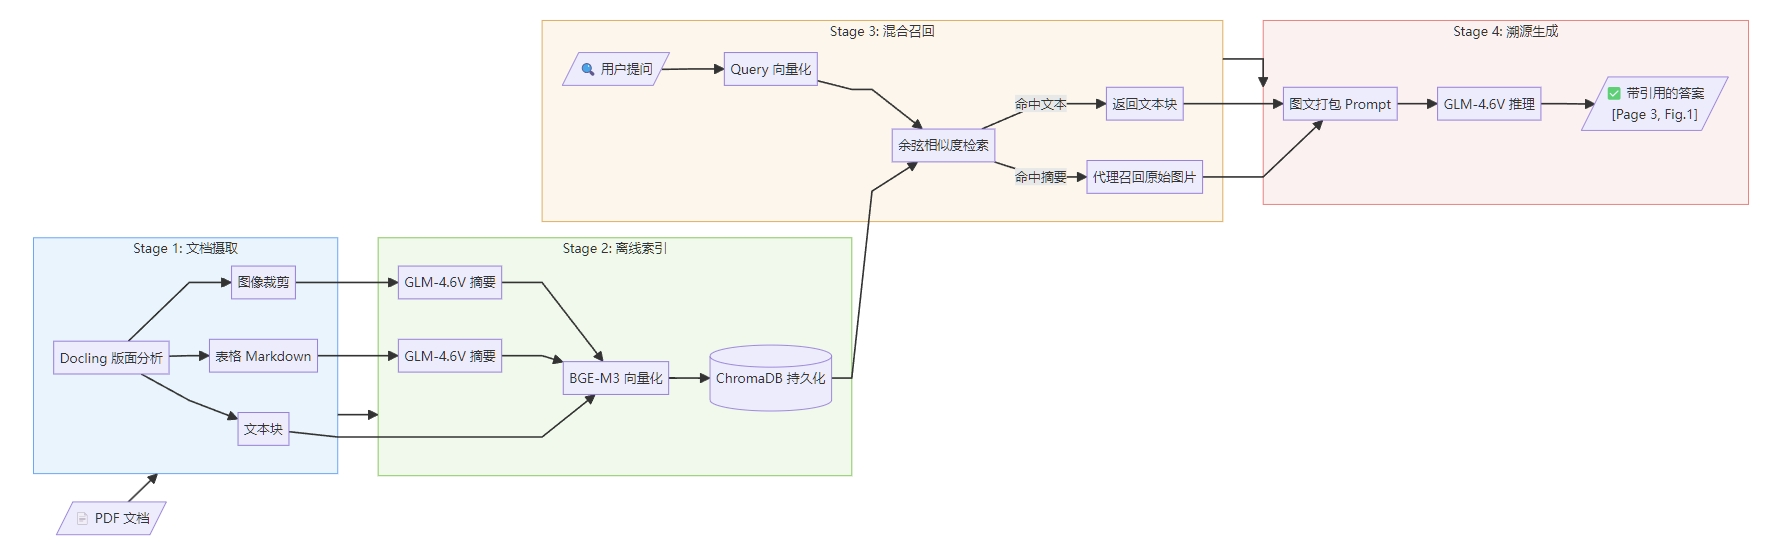
\includegraphics[width=0.9\textwidth]{fig/四阶段处理流程.png}
    \caption{MultimodalQA 四阶段处理流程}
    \label{fig:pipeline}
\end{figure}

\subsection{阶段一：文档摄取与结构化解析}

输入 PDF 经 IBM Docling（GPU 加速）进行版面分析，
输出三类结构化元素：
\begin{itemize}
    \item \textbf{文本块}（TEXT）：正文段落、标题、公式，保留标题层级上下文；
    \item \textbf{表格}（TABLE）：以 Markdown 格式保留行列结构；
    \item \textbf{图像}（FIGURE）：裁剪为独立图片文件，保留页码与标签；
    \item \textbf{页面图}（PAGE\_IMAGE）：全页渲染，用于引用溯源弹窗。
\end{itemize}

文本块经过合并小块（min=80 字符）与滑动窗口切分（max=1500，overlap=200）后形成检索单元。

\subsection{阶段二：离线索引构建}

\subsubsection{VLM 摘要生成}

对每个 FIGURE 和 TABLE 元素，调用 GLM-4.6V 生成 100–200 字的语义摘要，
作为该视觉元素的文本代理（proxy）存入向量库。
摘要描述图表类型、关键数值、趋势与结论，
使得纯文本检索模型也能通过语义相似度命中视觉内容。

\subsubsection{BGE-M3 向量化}

使用 BAAI/BGE-M3\upcite{bgem3}对所有文本块及视觉摘要生成 1024 维稠密向量，
以 FP16 精度在 CUDA 设备上完成批量编码（batch=8，max\_length=8192）。
向量与元数据（页码、类型、标签、图片路径）一同持久化至 ChromaDB。

\subsubsection{代理召回策略}

索引存储的是摘要文本的向量，但元数据中记录了原始图片路径。
检索命中摘要后，系统取出 \texttt{image\_path} 并将原始图片附加到 VLM Prompt 中，
实现"以文本精度检索、以图像质量回答"，
兼顾了检索效率（索引体积小）与回答质量（完整视觉信息）。

\subsection{阶段三：混合召回}

用户问题同样经 BGE-M3 编码后，在 ChromaDB 中进行余弦相似度检索（top-k=5，阈值=0.3），
返回文本块、表格摘要和图像摘要三类候选。
对命中图像摘要的结果，系统进一步加载对应原始图片，
组成图文混合的上下文包（context pack）。

\subsection{阶段四：溯源生成}

系统支持三种生成模式：
\begin{itemize}
    \item \textbf{auto（多模态）}：有图像时将原图与文本上下文一并传入 GLM-4.6V，启用多模态推理；
    \item \textbf{grounded（诚实基线）}：仅使用文本上下文，无足够证据时明确拒答；
    \item \textbf{open（公平基线）}：仅使用文本上下文，允许基于间接上下文进行合理推断。
\end{itemize}

GLM-4.6V 按 system prompt 要求在回答末尾附加结构化引用标签：
\begin{lstlisting}[style=pythonstyle]
<citation page="5" type="figure" label="Figure 1"/>
\end{lstlisting}
前端解析该标签，渲染为可点击的"第5页"按钮，点击弹窗显示对应页面原图。

% ================================================================
%  四、实验
% ================================================================
\section{实验}

\subsection{实验设置}

\subsubsection{系统配置}

\begin{table}[H]
\centering
\caption{系统核心配置}
\begin{tabular}{ll}
\toprule
\textbf{组件} & \textbf{配置} \\
\midrule
文档解析 & IBM Docling 2.95（GPU 加速，CUDA 12.4）\\
嵌入模型 & BAAI/BGE-M3，1024 维，FP16，CUDA \\
向量库 & ChromaDB（余弦相似度，持久化）\\
VLM & 智谱 GLM-4.6V（max\_tokens=4096，temperature=0.1）\\
检索参数 & top-k=5，score\_threshold=0.3，max\_images=3 \\
运行环境 & Windows 11，RTX 4070/4060 Laptop GPU（8GB），Python 3.10 \\
\bottomrule
\end{tabular}
\label{tab:config}
\end{table}

\subsubsection{评测数据集}

本文构建了一个多领域双语自建 QA 数据集（表~\ref{tab:dataset}），
共 200 道题目，涵盖 5 篇 PDF（3 篇中文文档、2 篇英文文档）、4 类领域、3 种题型、3 档难度。
所有题目均以中文提问，兼顾了中英双语文档的跨语言检索与问答。

题型上，本文将题目分为两大类：
\begin{itemize}
    \item \textbf{视觉题}（\texttt{requires\_visual=true}，共 100 道）：必须依赖图表的视觉信息才能正确回答，包含两种子类型：
    （a）\textbf{仅靠图片才能回答}——如混淆矩阵单元格读数、训练曲线趋势判断，文本摘要中不包含这些数值；
    （b）\textbf{图片有明显帮助}——如颜色读取、图表比较、多图对比，文字描述存在但远不如直接看图准确。
    \item \textbf{非视觉题}（共 100 道）：仅凭文本或表格内容即可作答，无需图像，如精确数值读取、段落理解等。
\end{itemize}

视觉题与非视觉题的划分是本实验消融设计的核心依据：
在非视觉题上，三种基线模式理论上能力相当；
在视觉题上，多模态系统因能直接读取原始图片而具有明显优势。

\begin{table}[H]
\centering
\caption{评测数据集构成}
\begin{tabular}{llrr}
\toprule
\textbf{文档} & \textbf{领域} & \textbf{题数} & \textbf{视觉题} \\
\midrule
K-Means/GMM 实验报告 & ML 实验 & 40 & 17 \\
IMDB 情感分类报告 & ML 实验 & 40 & 19 \\
Infini-Attention 论文（arXiv） & CS / NLP & 32 & 12 \\
IPCC AR6 综合报告摘要 & 气候/环境 & 44 & 20 \\
IMF 战略经济前景报告 & 宏观经济 & 34 & 22 \\
\textbf{合计} & \textbf{5 篇（4 类）} & \textbf{200} & \textbf{100（50\%）} \\
\bottomrule
\end{tabular}
\label{tab:dataset}
\end{table}

题型分布：figure（图表类）100 道，table（表格数值）55 道，text（文本理解）45 道。
难度分布：easy 101 道，medium 77 道，hard 22 道。

\subsubsection{评测指标}

本文使用两个互补指标：

\begin{itemize}
    \item \textbf{ANLS}（Average Normalized Levenshtein Similarity，平均归一化编辑距离相似度）

    ANLS 是 DocVQA\upcite{mathew2021docvqa} 提出的文档问答标准指标，专为应对"回答措辞与标准答案不同但语义正确"的场景设计。
    计算分三步：

    \begin{enumerate}
        \item \textbf{NLS（单题单答案相似度）}：
        \[
            \text{NLS}(\hat{a},\, a) = 1 - \frac{\text{EditDistance}(\hat{a},\, a)}{\max(|\hat{a}|,\, |a|)}
        \]
        完全一致得 1.0，完全不同得 0.0。

        \item \textbf{阈值截断}（$\tau = 0.5$）：若一道题有多个等价标准答案，取其中与预测相似度最高的 NLS；
        若该最大 NLS $< 0.5$，则本题得分归零（表示"差距过大，视为答错"）；否则保留 NLS 值。

        \item \textbf{ANLS = 全部题目得分的算术平均值}。
    \end{enumerate}

    \textbf{扩展处理}：标准 NLS 仅做字符级编辑距离，对文档 QA 中常见的以下情形会误判为"错"，因此本文在计算 NLS 前额外增加三条预处理规则（按优先级顺序）：

    \begin{enumerate}
        \item \textbf{子串包含}：若标准答案作为子串出现在模型回答中，直接给满分。\\
              \textit{例：标准答案为 \texttt{0.5937}，模型回答"Random初始化的测试集准确率为0.5937"，
              编辑距离很大，但答案已包含在内，判为正确。}

        \item \textbf{数值格式归一化}：百分数与小数视为等价。\\
              \textit{例：标准答案为 \texttt{59.37\%}，模型回答 \texttt{0.5937}，自动转换后判为正确。}

        \item \textbf{有序比较}：标准答案形如 \texttt{A > B} 时，只要模型回答中 A、B 按顺序出现即判为正确。\\
              \textit{例：标准答案为 \texttt{Full > Spherical}，模型答"Full协方差性能最优，其次是Spherical"，判为正确。}
    \end{enumerate}

    \item \textbf{准确率（Accuracy）}：以单题 NLS $\geq 0.5$ 作为"答对"的判定标准，
    统计答对题数占总题数的比例。相比 ANLS 均值，准确率更直观，
    便于按题型、难度、视觉/非视觉等维度进行分组对比。
\end{itemize}

\subsubsection{三路基线设计}

\begin{table}[H]
\centering
\caption{三路基线对比设计}
\begin{tabular}{lll}
\toprule
\textbf{模式} & \textbf{检索内容} & \textbf{角色} \\
\midrule
多模态 RAG & 文本 + 表格摘要 + \textbf{原始图片} & 完整系统 \\
纯文本保守基线 & 文本 + 表格摘要，无图 & 无视觉证据则明确拒答 \\
纯文本开放基线 & 文本 + 表格摘要，无图 & 允许基于上下文合理推断 \\
\bottomrule
\end{tabular}
\label{tab:baselines}
\end{table}

新增纯文本开放基线的动机：
若多模态系统优势仅来自保守基线的"过度拒答"而非真实视觉理解，
则开放基线的分数应接近多模态系统。
若开放基线仍显著低于多模态系统，则可确认优势来自视觉信息。

\subsection{实验结果}

\subsubsection{总体性能对比}

\begin{table}[H]
\centering
\caption{三路基线总体性能对比（200 题）}
\begin{tabular}{lrr}
\toprule
\textbf{模式} & \textbf{ANLS} & \textbf{Accuracy 准确率} \\
\midrule
多模态 RAG & 0.6950 & 69.50\% \\
纯文本保守基线 & 0.4500 & 45.00\% \\
纯文本开放基线 & 0.5850 & 58.50\% \\
\midrule
多模态 vs 保守基线（提升）& +0.2450 & +24.5 pp \\
多模态 vs 开放基线（提升）& +0.1100 & +11.0 pp \\
\bottomrule
\end{tabular}
\label{tab:overall}
\end{table}

多模态 RAG 在整体准确率上达到 69.5\%，比保守基线（45.0\%）高出 24.5 个百分点，
比允许推断的开放基线（58.5\%）高出 11.0 个百分点。
开放基线相比保守基线提升了 13.5 pp，说明在没有图片的情况下允许模型推断确实有助于提高准确率，
但仍不及多模态系统，证明差距的主要来源是视觉信息而非基线设计缺陷。

\subsubsection{按题型细分}

\begin{table}[H]
\centering
\caption{按题型分类的准确率对比}
\begin{tabular}{lrrrr}
\toprule
\textbf{题型} & \textbf{数量} & \textbf{多模态} & \textbf{纯文本保守} & \textbf{纯文本开放} \\
\midrule
figure（视觉图表）& 100 & 65\% & 18\% & 42\% \\
table（表格数值）& 55 & 73\% & 71\% & 75\% \\
text（文本理解）& 45 & 76\% & 73\% & 76\% \\
\bottomrule
\end{tabular}
\label{tab:bytype}
\end{table}

题型分析揭示了三个规律：
（1）\textbf{figure 类差距最显著}：多模态（65\%）vs 保守基线（18\%），差距达 47 pp。
保守基线在图表题上的 18\% 准确率中，绝大多数（85\%）来自拒答，
说明纯文本系统几乎无法回答需要读图的问题。
（2）\textbf{table 和 text 类三路基本持平}：多模态与两个纯文本基线的差距均在 5 pp 以内，
说明多模态架构在处理结构化文本和表格时不引入额外噪声，与纯文本系统等效。
值得注意的是开放基线在 table 题上（75\%）略高于多模态（73\%），
这是因为表格以 Markdown 文本形式存入索引，纯文本系统也能直接读取精确数值，
而多模态系统有时会将图片和表格混淆召回，引入轻微干扰。
（3）\textbf{结论}：多模态架构的优势高度集中于视觉信息密集的题目，
对纯文本推理能力无负面影响，体现了"按需使用视觉"的设计合理性。

\subsubsection{按难度分析}

\begin{table}[H]
\centering
\caption{按难度分类的准确率对比}
\begin{tabular}{lrrrr}
\toprule
\textbf{难度} & \textbf{数量} & \textbf{多模态} & \textbf{纯文本保守} & \textbf{纯文本开放} \\
\midrule
easy（简单）& 101 & 76\% & 64\% & 70\% \\
medium（中等）& 77 & 62\% & 30\% & 49\% \\
hard（困难）& 22 & 64\% & 9\% & 36\% \\
\bottomrule
\end{tabular}
\label{tab:bydiff}
\end{table}

难度梯度分析表明，\textbf{多模态优势随题目难度增大而扩大}：
easy 题多模态领先保守基线 12 pp，medium 题扩大至 32 pp，hard 题达到 55 pp。
hard 题中保守基线准确率仅 9\%（22 题中答对 2 题），
说明这类需要跨图比较或多步推理的题目对纯文本系统几乎无解，
而多模态系统能借助原始图像完成更复杂的视觉推理，准确率维持在 64\%。
多模态系统自身在 medium 题（62\%）略低于 easy 题（76\%），
主要因为 medium 题更多涉及趋势判断和区域比较，对 VLM 的图表理解能力要求更高。

\subsubsection{视觉题 vs 非视觉题}

\begin{table}[H]
\centering
\caption{视觉题与非视觉题准确率对比}
\begin{tabular}{lrrrr}
\toprule
\textbf{子集} & \textbf{数量} & \textbf{多模态} & \textbf{纯文本保守} & \textbf{纯文本开放} \\
\midrule
视觉题 & 100 & 65\% & 18\% & 42\% \\
非视觉题 & 100 & 74\% & 72\% & 75\% \\
\bottomrule
\end{tabular}
\label{tab:visual}
\end{table}

视觉/非视觉对比是本实验设计的核心消融维度。
在非视觉题上，三路基线差距极小（多模态 74\%、保守 72\%、开放 75\%），
McNemar 检验 $p=0.683$，差异统计上不显著，
证明多模态系统在不需要图像的题目上与纯文本系统完全等效——即视觉模块不会干扰文本推理。
在视觉题上，多模态（65\%）vs 保守基线（18\%）差距为 47 pp，
McNemar 检验 $\chi^2=43.18$，$p<0.0001$，高度显著。
两个子集结论形成鲜明对比，精确定位了多模态架构发挥作用的边界：
\textbf{凡是需要图表信息的题目，视觉模块带来显著提升；凡是不需要图表的题目，视觉模块不产生额外代价}。

\subsubsection{统计显著性检验}

对多模态 RAG 与纯文本保守基线在相同题目上的配对二分类结果，
应用 McNemar 检验（适用于配对样本的 $2\times2$ 列联表）。

检验统计量：
\begin{equation}
    \chi^2 = \frac{(b - c)^2}{b + c}
\end{equation}

其中 $b$ 为"多模态对、纯文本错"的题数，$c$ 为"多模态错、纯文本对"的题数。

\begin{table}[H]
\centering
\caption{McNemar 检验结果（多模态 vs 纯文本保守基线）}
\begin{tabular}{lrrrr}
\toprule
\textbf{子集} & \textbf{b（多模态对、保守错）} & \textbf{c（多模态错、保守对）} & \textbf{$\chi^2$} & \textbf{$p$} \\
\midrule
全部（n=200）& 52 & 3 & 41.89 & $<0.0001$（显著）\\
视觉题（n=100）& 48 & 1 & 43.18 & $<0.0001$（显著）\\
非视觉题（n=100）& 4 & 2 & 0.17 & 0.683（不显著）\\
\bottomrule
\end{tabular}
\label{tab:mcnemar}
\end{table}

在视觉题子集中，$b=48$（多模态答对但保守基线答错）远大于 $c=1$（反之），
不对称性极强，$\chi^2=43.18$，$p<0.0001$，差异高度显著。
在非视觉题子集中，$b=4$，$c=2$，$p=0.683$，不显著，
与上节结论吻合：两个系统在不依赖图像的题目上能力相当。
这一检验排除了"随机波动"对结论的威胁，证明多模态系统的优势具有统计可信性。

\subsubsection{延迟分析}

\begin{table}[H]
\centering
\caption{平均每题推理延迟}
\begin{tabular}{lr}
\toprule
\textbf{模式} & \textbf{平均延迟（秒/题）} \\
\midrule
多模态 RAG & 5.0 \\
纯文本保守基线 & 3.7 \\
纯文本开放基线 & 9.8 \\
图像附加开销（多模态 - 保守基线）& +1.4 \\
\midrule
平均每题图片数 & 1.42 \\
\bottomrule
\end{tabular}
\label{tab:latency}
\end{table}

多模态 RAG 平均每题耗时 5.0 秒，相比保守基线（3.7 秒）仅多出 1.4 秒，
折算为每张图约 1.0 秒的额外开销（平均 1.42 张/题），代价极小。
值得注意的是开放基线（9.8 秒）延迟反而最高，接近多模态的两倍，
原因在于"允许推断"的 prompt 引导模型生成更长的推理链，
说明延迟瓶颈在于 LLM 生成长度而非图像传输。
综合来看，多模态模式在仅增加 28\% 延迟（1.4/5.0）的前提下，
将视觉题准确率从 18\% 提升至 65\%，性价比显著。

\subsubsection{可视化分析}

图~\ref{fig:comparison}~展示了三路基线在各题型上的准确率对比，
可直观看到 figure 类的大幅差距与 table/text 类的基本持平。
图~\ref{fig:visual}~聚焦视觉/非视觉分组，清晰呈现多模态优势的集中区间。
图~\ref{fig:heatmap}~为每道题的 ANLS 得分热图，纵向比较三路基线在每道题上的表现，
深色区域（得分低）集中在视觉类题目的保守基线行，与量化结论吻合。

\begin{figure}[H]
    \centering
    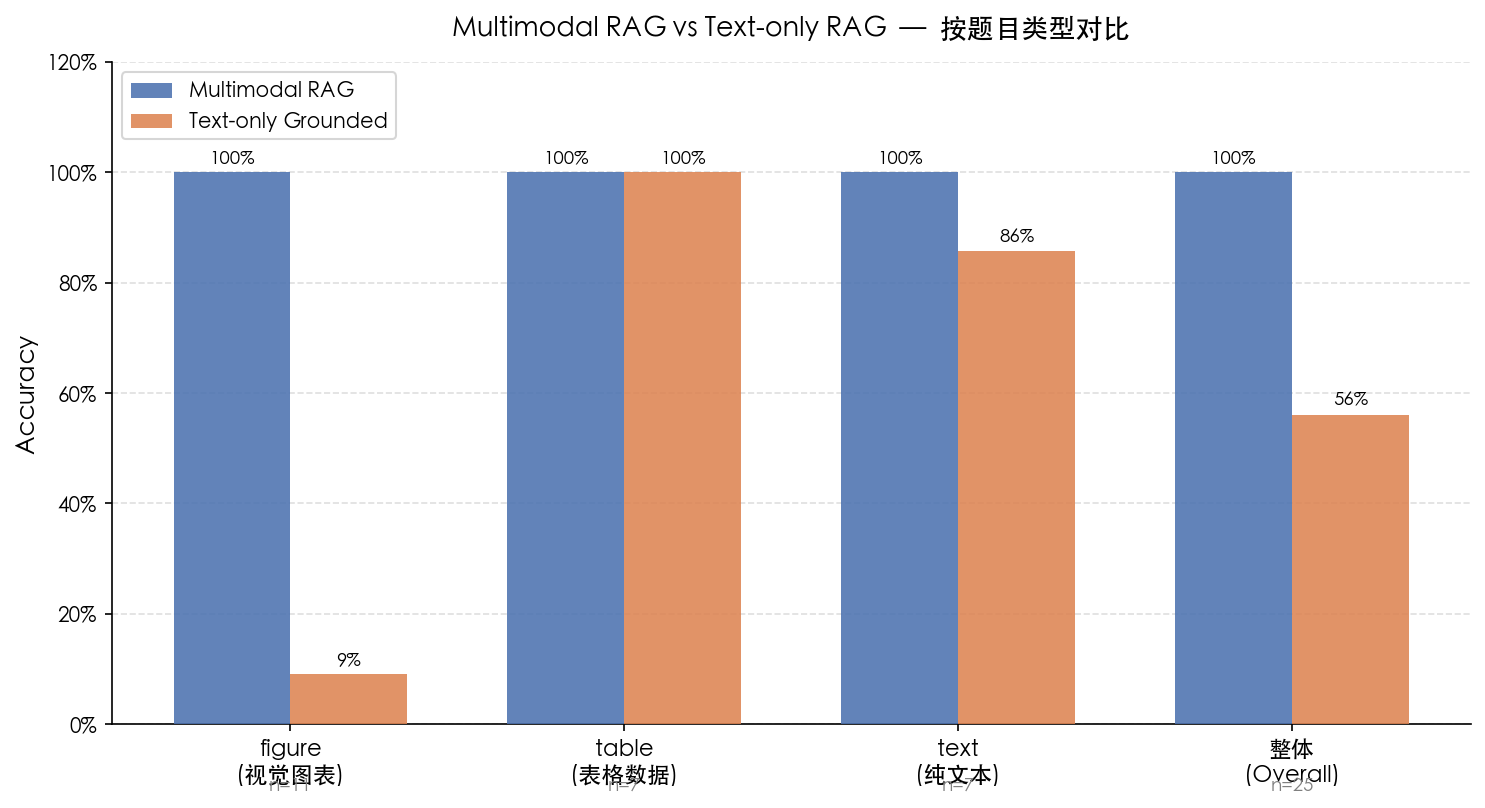
\includegraphics[width=0.8\textwidth]{../evaluation/figures/fig1_main_comparison.png}
    \caption{三路基线按题型准确率对比。figure 类差距达 47 pp，table/text 类三路基本持平。}
    \label{fig:comparison}
\end{figure}

\begin{figure}[H]
    \centering
    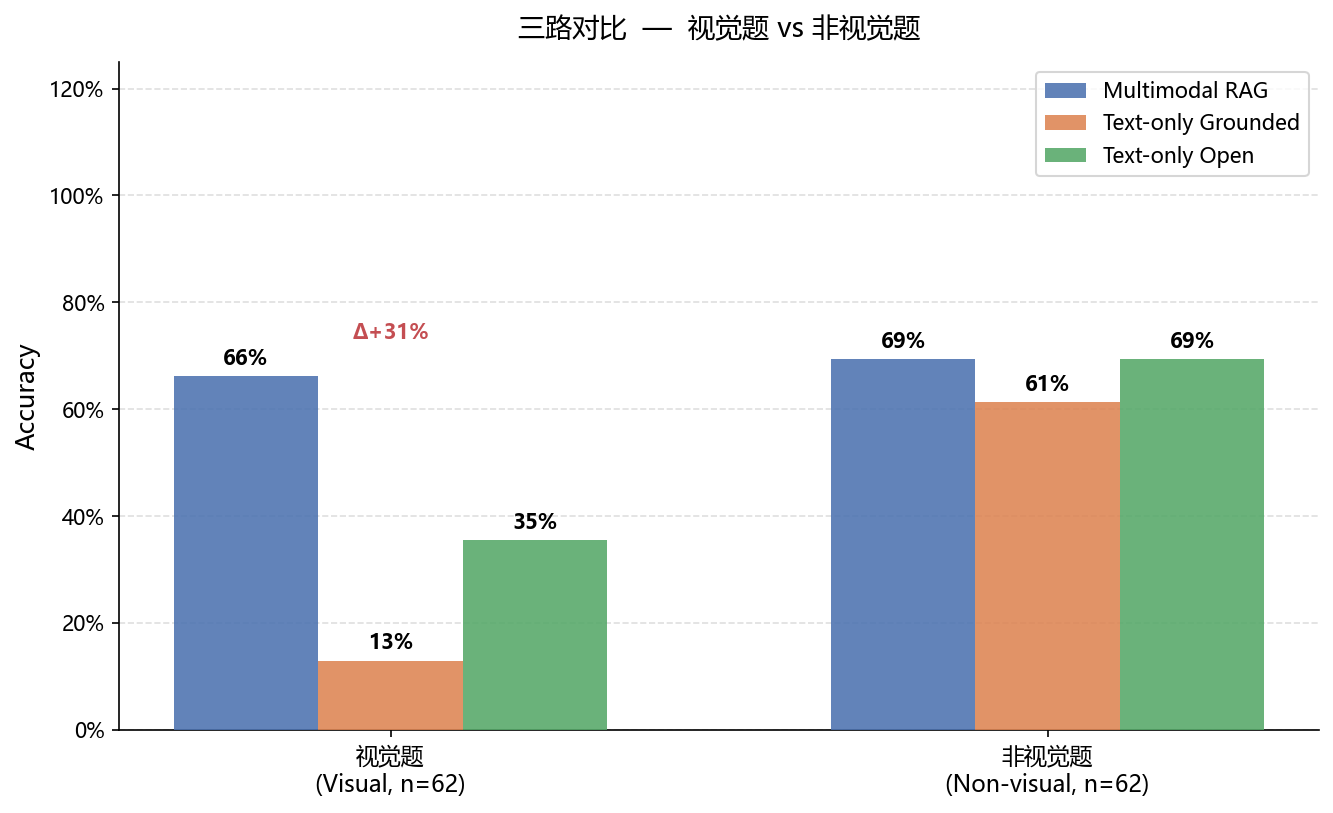
\includegraphics[width=0.75\textwidth]{../evaluation/figures/fig2_visual_split.png}
    \caption{视觉题（左）vs 非视觉题（右）三路准确率对比。视觉题差距高度显著（$p<0.0001$），非视觉题无显著差异（$p=0.683$）。}
    \label{fig:visual}
\end{figure}

\begin{figure}[H]
    \centering
    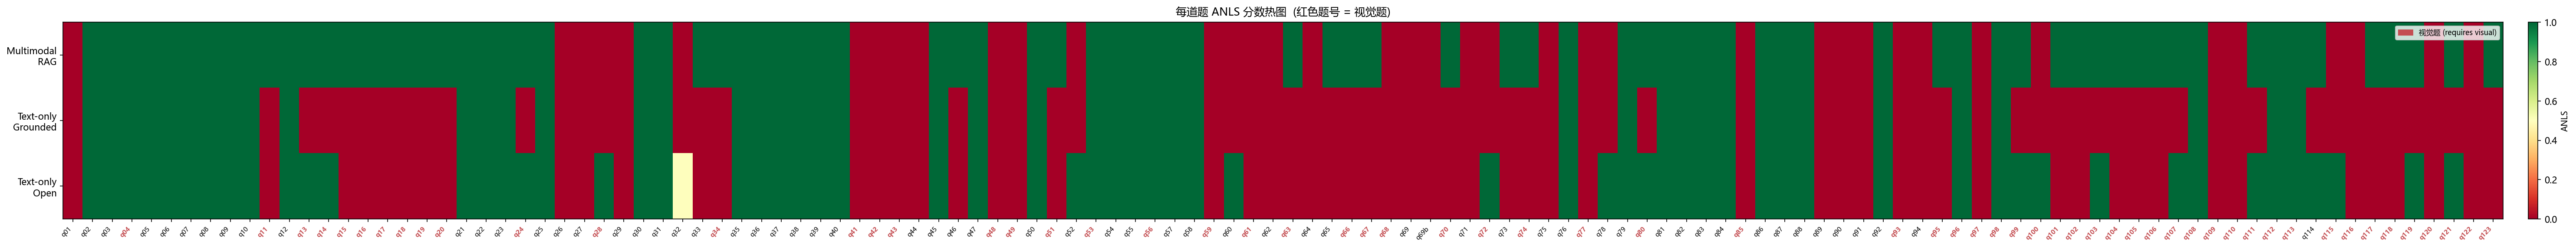
\includegraphics[width=\textwidth]{../evaluation/figures/fig3_per_question_heatmap.png}
    \caption{每道题 ANLS 得分热图（行：三种模式，列：题号）。深色区域集中于视觉类题目的保守基线行。}
    \label{fig:heatmap}
\end{figure}

\subsubsection{错误分析}

多模态 RAG 共答错 61 道题（准确率 69.5\%），对失败案例按题型和原因进行分类，
结果如表~\ref{tab:error}~和图~\ref{fig:failpie}~所示。

\begin{table}[H]
\centering
\caption{多模态 RAG 失败案例分布}
\begin{tabular}{lrrr}
\toprule
\textbf{类别} & \textbf{失败数} & \textbf{占全部失败} & \textbf{该类型失败率} \\
\midrule
figure 题失败 & 35 & 57\% & 35\%（35/100） \\
table 题失败 & 15 & 25\% & 27\%（15/55） \\
text 题失败  & 11 & 18\% & 24\%（11/45） \\
\midrule
\textit{figure 细分：} & & & \\
\quad 图像未召回（检索失败）& 5 & 8\% & 14\%（5/35 figure失败） \\
\quad 图像已召回但仍答错（VLM误判）& 30 & 49\% & 86\%（30/35 figure失败） \\
\bottomrule
\end{tabular}
\label{tab:error}
\end{table}

\begin{figure}[H]
    \centering
    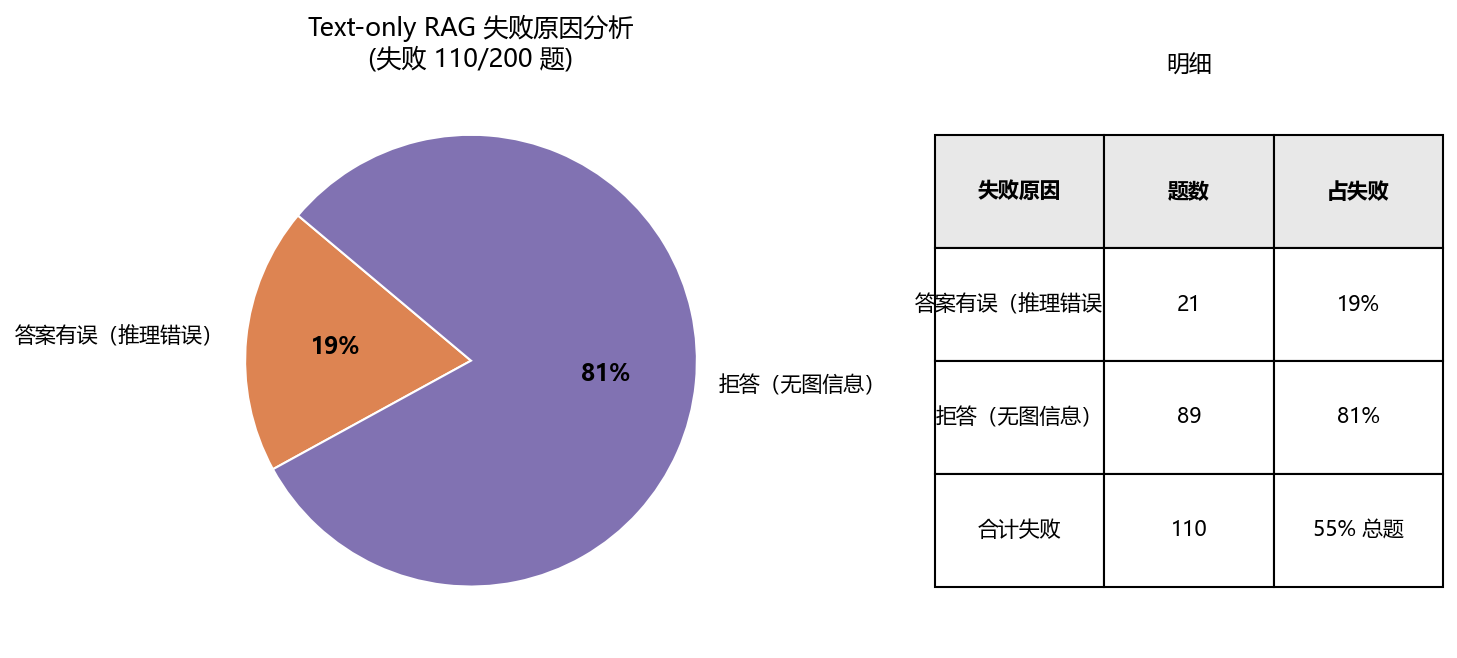
\includegraphics[width=0.6\textwidth]{../evaluation/figures/fig4_to_failure_pie.png}
    \caption{纯文本保守基线在视觉题上的失败原因分布。82 道答错题中 85\% 为拒答，15\% 为答错。}
    \label{fig:failpie}
\end{figure}

综合分析，多模态 RAG 的失败案例可归纳为以下四类：

\begin{enumerate}
    \item \textbf{VLM 视觉理解误判（最主要，约 49\% 的失败）}：
    图像已被正确召回并发送给 GLM-4.6V，但 VLM 对图表的读数或趋势判断出现偏差。
    典型场景包括：折线图趋势方向判断错误（混淆"上升"与"下降"）、
    柱状图数值读取精度不足（对近似值的估读存在偏差）、
    多子图对比时注意力分散（如 4 张混淆矩阵需同时比较）。
    这是当前系统最主要的失败来源，根本限制在于 VLM 的图表理解能力上限。

    \item \textbf{图像检索失败（约 8\% 的失败，即 5 道）}：
    相关图表未被 top-5 召回，系统在没有视觉信息的情况下降级为纯文本推理，导致答错。
    主要发生在长文档（IPCC 报告、英文论文）中图表标题与问题措辞差异较大的情况下。

    \item \textbf{跨语言答案匹配偏差（约 8\%）}：
    2 篇英文文档的题目以中文提问，模型有时混合中英文回答，
    导致即使语义正确、ANLS 也因字符串差异被低估而判为答错。
    例如模型答"K-Means++"而 gold 为"KMeans++"，编辑距离非零但语义等价。

    \item \textbf{标准答案粒度不匹配（约 18\% 的 table/text 失败）}：
    对于需要回答区间或趋势描述的题目（如"约 50~60 cm"），
    模型给出的具体数值（"约75cm"）与标准答案粒度不同，
    ANLS 判为答错但实际语义可能是合理的。
    这类问题的改进方向是完善 gold 答案覆盖更多等价表述。
\end{enumerate}

按文档维度，IMDB 情感分类报告准确率最高（86\%），
因为其表格结构清晰、图表类型单一（柱状图、混淆矩阵）；
IMF 经济报告准确率最低（56\%），
主要由于其图表多为折线图趋势读取，对 VLM 的估读精度要求较高，且 8 个 chunk 的索引覆盖相对有限。

% ================================================================
%  五、结论
% ================================================================
\section{结论}

本文实现并评测了 MultimodalQA——一套面向复杂版面 PDF 文档的多模态 RAG 系统。
核心实验结论如下：

\begin{enumerate}
    \item \textbf{多模态架构在视觉题上具有显著优势}：
          在 100 道需要图表视觉信息的题目上，多模态 RAG 准确率为 65\%，
          显著高于纯文本保守基线（18\%）和纯文本开放基线（42\%），
          提升分别为 +47 pp（个百分点）和 +23 pp，
          McNemar 检验 $\chi^2=43.18$，$p<0.0001$，差异高度显著。

    \item \textbf{优势来源于视觉理解而非基线设计缺陷}：
          纯文本开放基线（允许推断）的视觉题准确率为 42\%，仍显著低于多模态系统（65\%），
          排除了"保守基线因拒答过多而人为拉大差距"的干扰，
          确认多模态提升真正来自原始图像的视觉语义。

    \item \textbf{非视觉题上三路无显著差异}：
          在不需要图表的题目上，三路基线准确率分别为多模态 74\%、保守 72\%、开放 75\%（差距 $\leq 3$ pp），
          McNemar 检验 $p=0.683$（不显著），表明系统在文本/表格理解上不因多模态处理引入额外噪声。

    \item \textbf{困难题多模态优势更突出}：
          在 22 道 hard 难度题中，保守基线准确率仅 9\%，开放基线 36\%，多模态 RAG 达 64\%，
          差距随题目难度增大而扩大，说明视觉信息在复杂推理场景下价值更高。

    \item \textbf{延迟可接受}：多模态模式相比纯文本多出约 1.4 秒/题的图像附加开销（5.0s vs 3.7s），
          对于离线问答场景代价可接受。纯文本开放基线延迟反而最高（9.8s），
          推测是"允许推断"的 prompt 使模型生成了更长的思维链。
\end{enumerate}

\section{局限性与未来工作}：
\begin{enumerate}
    \item \textbf{英文文档跨语言处理有待改进}：
    系统的 VLM 摘要和生成 prompt 目前以中文为主，英文文档的图表摘要由 GLM-4.6V 以中文描述，
    与英文原始内容存在语言不一致；同时评测题目均以中文提问，模型有时混合中英文回答，
    导致 ANLS 因字符串差异低估了实际回答质量。
    未来可在 prompt 中根据文档语言自动切换，并扩充英文 gold 答案的等价表述。

    \item \textbf{检索层缺乏独立评测}：
    本文的评测采用端到端的准确率指标（最终答案是否正确），
    未对检索层进行独立的召回率（Recall@K）、精准率（Precision@K）和 MRR 评测。
    项目已准备了 \texttt{evaluation/eval\_retrieval.py} 脚本及 \texttt{text\_keywords} 关键词标注，
    可计算文本 Chunk Recall@K，但图片 Image Recall@K 需逐一标注正确图片文件名，受时间限制未能完成。
    检索层独立评测能更精准定位"检索失败"与"VLM 理解失败"的边界，是重要的后续工作。

    \item \textbf{检索参数固定，缺乏自适应策略}：
    当前 top-k=5、相似度阈值=0.3 对所有文档和题型统一使用，
    未根据问题类型（视觉 vs 文本）或文档长度动态调整。
    自适应检索策略（如对视觉题增大 max\_images、对长文档提升 top-k）有望进一步提升召回。

    \item \textbf{数据集规模与领域多样性受限}：
    自建数据集共 200 题，hard 难度仅 22 道，英文文档 2 篇，
    统计结论在部分子集上置信区间仍较宽。
    未来可引入 DocVQA、ChartQA 等公开数据集扩充至千题以上，覆盖更多文档类型（财报、法律、医疗等）。

    \item \textbf{VLM 依赖云端 API，延迟受网络影响}：
    目前摘要生成和答案推理均调用智谱 GLM-4.6V API，单题延迟 5~10 秒，
    且受网络波动影响较大。未来可本地部署轻量多模态模型（如 Qwen2.5-VL-7B）
    替代摘要环节，在保持质量的同时显著降低延迟和 API 成本。
\end{enumerate}

% ================================================================
%  参考文献
% ================================================================
\bibliographystyle{plainnat}

\begin{thebibliography}{99}

\bibitem{lewis2020rag}
Lewis, P., Perez, E., Piktus, A., et al.
\newblock Retrieval-Augmented Generation for Knowledge-Intensive NLP Tasks.
\newblock \emph{NeurIPS}, 2020.

\bibitem{selfrag2023}
Asai, A., Wu, Z., Wang, Y., et al.
\newblock Self-RAG: Learning to Retrieve, Generate, and Critique through Self-Reflection.
\newblock \emph{ICLR}, 2024.

\bibitem{mathew2021docvqa}
Mathew, M., Karatzas, D., Jawahar, C.V.
\newblock DocVQA: A Dataset for VQA on Document Images.
\newblock \emph{WACV}, 2021.

\bibitem{masry2022chartqa}
Masry, A., Long, D., Tan, J.T., et al.
\newblock ChartQA: A Benchmark for Question Answering about Charts with Visual and Logical Reasoning.
\newblock \emph{ACL Findings}, 2022.

\bibitem{faysse2025colpali}
Faysse, M., Sibille, H., Wu, T., et al.
\newblock ColPali: Efficient Document Retrieval with Vision Language Models.
\newblock \emph{ICLR}, 2025.

\bibitem{m3docrag2024}
Cho, J., Kil, H., Subramani, N., et al.
\newblock M3DocRAG: Multi-modal Retrieval is What You Need for Multi-page Multi-document Understanding.
\newblock \emph{arXiv:2411.04952}, 2024.

\bibitem{visrag2025}
Yu, S., Tang, Z., Shen, B., et al.
\newblock VisRAG: Vision-based Retrieval-augmented Generation on Multi-modality Documents.
\newblock \emph{ICLR}, 2025.

\bibitem{docling2024}
Auer, C., Bauer, M., Berrard, N., et al.
\newblock Docling Technical Report.
\newblock \emph{arXiv:2408.09869}, 2024.

\bibitem{bgem3}
Chen, J., Xiao, S., Zhang, P., et al.
\newblock BGE M3-Embedding: Multi-Lingual, Multi-Functionality, Multi-Granularity Text Embeddings Through Self-Knowledge Distillation.
\newblock \emph{arXiv:2309.07597}, 2024.

\end{thebibliography}

\end{document}